\section{Computer Simulations}

The theory of classical mechanics is often regarded as the first major breakthrough in
the field of physics. For every aspiring physicist this is still the starting point of
their studies. Unfortunately, getting to know these relatively simple laws of nature
leads to the inescapable realisation that these theories are expressed in mathematical
formalisms that are only analytically solvable in few idealised scenarios. Applying these
formulas to a problem consisting of just more then two particles already leads to
practically unsolvable equations.

Although it is often not possible to find an exact solution to equations
related to complex physical systems, finding reasonable approximations to their solution
is achievable. One popular method to analyse the dynamics of complex systems is the use
of computer simulations.

\begin{wrapfigure}[20]{r}{0.5\textwidth}
    \vspace{-0.5cm}
  \begin{center}
    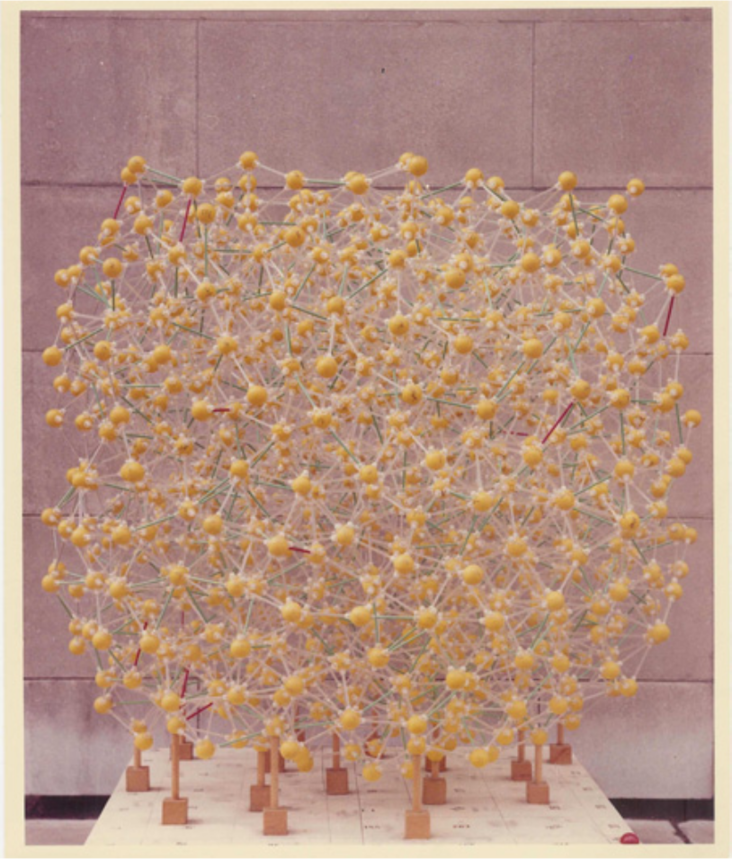
\includegraphics[width=0.4\textwidth]{Figures/WaterModel.png}
  \end{center}
  \caption[Example of an expanded model of a simple liquid.]{Example of an expanded model
  of a simple liquid (J L Finney, Ph.D thesis).
  \cite{Finney_2007}}
\end{wrapfigure}

Simulations have a rich history within physics and engineering, starting even before the
invention of the computer. An example of one of these mechanical simulations is the
'Waterloopkundig Laboratorium', a hydrological laboratory located in Delft
\cite{Vreugdenhil2001}.  This
laboratory houses a scale model of important Dutch waterways, where the influence of
waves on harbours and docks was studied.  The simulation provided revolutionary insights
into the behaviour of water and played an important part in the design of the famous
Delta Works.

Another more topical example is the use of mechanical simulations to study the
structure of water.  In the early 20th century Prof. J.D. Bernal and his fellow
researchers built various ball and stick models of water to analyse the possible 3D
configurations of water molecules in a liquid \cite{Finney_2007}. Their research
eventually explained the peculiar physical properties of water from an atomistic
perspective. Despite how useful these mechanical simulations turned out to be, the
biggest drawback of the method was the extreme cost of labour involved with their
construct. As Prof. Bernal alluded to in his famous 1962 lecture,

\begin{quote}
\dots I took a number of rubber balls and stuck them together with rods of a
selection of different lengths ranging from 2.75 to 4 inch. I tried to do this in the
first place as casually as possible, working in my own office being interrupted every
five minutes or so and not remembering what I had done before the interruption.\dots
\cite{Bernal1962}
\end{quote}

After the first computer simulations where performed in the Los Alamos laboratory
\cite{Metropolis1953}, the
popularity of simulations rapidly increased. The remarkable explanatory power of
simulations, combined with the relative easy construction of computer models, led to a
fast adoption of computer simulations in the scientific community. Within the context of
this thesis, computer simulations are used to study the mechanics of
the DNA polymer. Due to the high number of atoms in a typical system it is generally
not possible to find an analytical solution to their equations of motion. In this
context simulations are often used to gain an insight into the complex dynamics of the
system and guide the developments of more simple approximate theories. The simulations
act as a bridge between the microscopic constituents of the systems and the macroscopic
properties we want to understand.

\subsection{Molecular Dynamics Simulations}
Molecular Dynamics (MD) is a computer simulation technique, used to analyse
the dynamics of a classical many-body system. The central idea of this method is to
generate all the trajectories in a system of $N$ particles by numerically
integrating the classical equations of motion,
\[
m_i \frac{d^2 \boldsymbol{r_i}}{dt^2} = \boldsymbol{f_i}, \quad \boldsymbol{f_i} = -
    \frac{\partial}{\partial \boldsymbol{r_i}} \mathcal{U}, \quad for\ i \in N.
\]
The motion of the particles are governed by the forces $f_i$ acting upon them, which are
usually derived from the interaction potential $\mathcal{U}$.
Solving these differential equations is achieved by employing a discretized time
integration scheme. The discretization resolution is conventionally called the time step
of the simulations denoted by $\Delta t$. A typical molecular dynamics scheme is shown in
Algorithm 1.

There are a large number of different integrations schemes that one can choose
from, in which the choice depends entirely on the system at hand.
When working with an isolated system -- i.e. microcanonical ensemble --, logically an
energy conserving integrator is needed. The canonical
choice for this type of integration scheme is the Velocity-Verlet algorithm. This
algorithm is an example of leapfrog integration, where the updating of the positions
and velocities are interleaved at different points in time. The major strength of this
type of algorithm is that it turns out to be a symplectic integrator. This means that the
errors on the total energy due to discretization are bounded.

On the other hand, when a system is in contact with a thermal reservoir --i.e. canonical
ensemble-- the total energy is not conserved, but rather the temperature of the
simulation should be fixed. To achieve this a thermostat is implemented in the MD
simulation. A typical thermostat attempts to negate any drift in temperature by
appropriately importing or exporting energy to the system after each time step.
Popular examples of thermostats are the Nos\'e-Hoover thermostat or the Langevin
thermostat. The latter regulates the temperature by introducing an implicit solvent to
the simulation that gives rise to random thermal kicks. The resulting equations of motion
are the Langevin equations given by,

\begin{equation}
    m_i \frac{d^2 \boldsymbol{r}_i}{dt^2} = - \nabla \mathcal{U} - \gamma_i \frac{d
    \boldsymbol{r}_i}{d t} +
    \xi_i(t),
\end{equation}
where $\gamma_i$ is known  as the friction coefficient and $\xi_i(t)$ a stochastic force
acting upon the particles. The combination of the last two terms fully capture the
statistical consequences of the solvent interacting with the system.

\begin{algorithm}
    \SetKwFunction{isOddNumber}{isOddNumber}
    \SetKwInOut{KwIn}{Input}

    \KwIn{Initial configuration of all atoms ($\boldsymbol{r}$, $\boldsymbol{v}$,
    $\boldsymbol{a}$) and choose short  $\Delta t$ }
    % $call\ init \gets [\boldsymbol{r}$, $\boldsymbol{v}$,
    % $\boldsymbol{a}]$\\
    % $t \gets 0$\\
    \tcc{Initialising the simulation}
    \textbf{setup} initial conditions\\
    \textbf{set} $t \gets 0$\\
    \tcp{}
    \tcc{Running the MD loop}

    \While{$t\ \leq\ t_{max}$}
    {
      % f \get $call\ force(state)$ \tcp*[f]{compute forces on all particles}\\
      % state \gets $call\ integrate(state, f)$ \tcp*[f]{integrate equations of motion}\\
      \textbf{compute} the forces on all particles\\
      \For {each particle}{
        \textbf{compute} new positions and momenta using an \textbf{integration scheme
      }}
       % $t \gets t+\Delta\ t$
      \textbf{update} $t \gets t+\Delta t$
    }
    \tcp{}
    \tcc{Output}
    \KwRet{final configuration of all atoms}
    \caption{Simple Molecular Dynamics Program}
\end{algorithm}

%
% \begin{center}
% 	\begin{tikzpicture}[
% 	squarednode/.style={rectangle, draw=blue!60, fill=blue!5, very thick, minimum width=50mm,
% 	minimum height=5mm},]
% 	%Nodes
% 	\node[squarednode]      (step1)                        {1};
% 	\node[squarednode]      (step2)       [below= 3mm of step1] {2};
% 	\node[squarednode]      (step3)       [below= 3mm of step2] {3};
% 	\node[squarednode]      (step4)       [below= 3mm of step3] {4};
% 	\node[squarednode]      (step5)       [below= 3mm of step4] {5};
% 	\node[squarednode]      (step6)       [below= 3mm of step5] {6};
% 	\node[squarednode]      (step7)       [below= 3mm of step6] {7};
% 	\node[squarednode]      (step8)       [below= 3mm of step7] {8};
%
% 	%Lines
%     \draw[very thick, ->] (step1.south) -- (step2.north);
% 	\draw[very thick, ->] (step2.south) -- (step3.north);
% 	\draw[very thick, ->] (step3.south) -- (step4.north);
% 	\draw[very thick, ->] (step4.south) -- (step5.north);
%     \draw[very thick, ->] (step5.south) -- (step6.north);
% 	\draw[very thick, ->] (step6.south) -- (step7.north);
% 	\draw[very thick, ->] (step7.south) -- (step8.north);
% 	\draw[very thick, ->] (step8.west)  -- +(-0.4,0) |-(step2.west);
% 	\end{tikzpicture}
% \end{center}



\subsection{Coarse Grained modelling}
As most things do, molecular dynamics simulations have their pitfalls. A commonly
encountered problem is the rapidly increasing computational cost when the number of
particles in the system increase. If not addressed, this would limit the scope of MD
simulations to systems of a few particles over short time-scales.

During these simulations the most costly calculations involve the non-bonded
interactions\footnote{Interactions acting between non-covalently bonded atoms. These
forces act both inter- and intramolecular, giving rise a large multiplicity in
interactions.} in the system. These interatomic interactions make the computational
complexity for rudimentary MD simulations scale as $O(N^2t)$, where $N$ is the number of
particles in the system and $t$ the simulation time. This bad scaling behaviour comes
arises from the fact that for each individual particle all the other particles are
contributing to its energy potential. To improve this scaling behaviour, the non-bonded
interactions in a MD simulation are almost always truncated. This localization of the
interatomic interactions has the favourable effect that not all atoms are involved in
every calculation. Efficient algorithms, like the multigrid method, have been derived
to improve the complexity of MD simulations to $O(Nt)$. \cite{Celeste2001}

From the scaling complexity we conclude that decreasing the total number of particles in
the system drastically improves the computational cost of an MD simulation. To reduce the
number of particles in a MD simulation a method called coarse-graining can be used.
In all atom simulations each atom is explicitly represented as a particle in the
simulation. Contrarily, coarse-grained simulation group together multiple atoms to form
generalised pseudo-atoms, with their respective pseudo-interaction. During this
simplification some atom details are neglected, resulting in a model that only
approximates our initial system. However, useful results can be obtained from
these simulations if we remain aware of the made approximations during the
simplification.

% Coarse graining is a method to further optimize molecular dynamics simulations.
% In all atom simulations each atom is explicitly represented as a particle in the
% simulation. Contrarily, coarse grained simulation use multiple atoms grouped
% together to form generalised pseudo-atoms, with their respective pseudo-interaction.

There are two distinctly different ways to construct a coarse grained model. The first
method starts from the all atom model of the system and generalises nearby atoms into
larger pseudo-atoms. This is called the bottom up approach. The top down approach, which
is the alternative method, focuses more on the precise reproduction of experimental
results. Here larger pseudo-atoms are designed based upon characteristic patterns in the
structure. Next the pseudo-interactions are tweaked to accurately reproduce the
system's dynamics.

In the field of DNA simulations coarse graining turned out to be a very important
method. Previously all atom simulations of DNA polymers were restricted to simulations of
less then hundred baisepairs over only a few microseconds. The development of
coarse-grained models allowed for the simulation of large scale systems, often
encountered in DNA technology. A few examples of commonly used coarse grained models of
DNA are Martini \cite{Souza2021}, 3SPN \cite{Freeman2011} and oxDNA
\cite{Ouldridge2010}.\\

\begin{figure}[ht]
  \begin{centering}
  \adjustbox{minipage=1.3em,valign=t}{\subcaption{}\label{sfig:testa}}%
  \begin{subfigure}[t]{\dimexpr.3\linewidth-1.3em\relax}
  \centering
  \vspace{-0.9cm}
  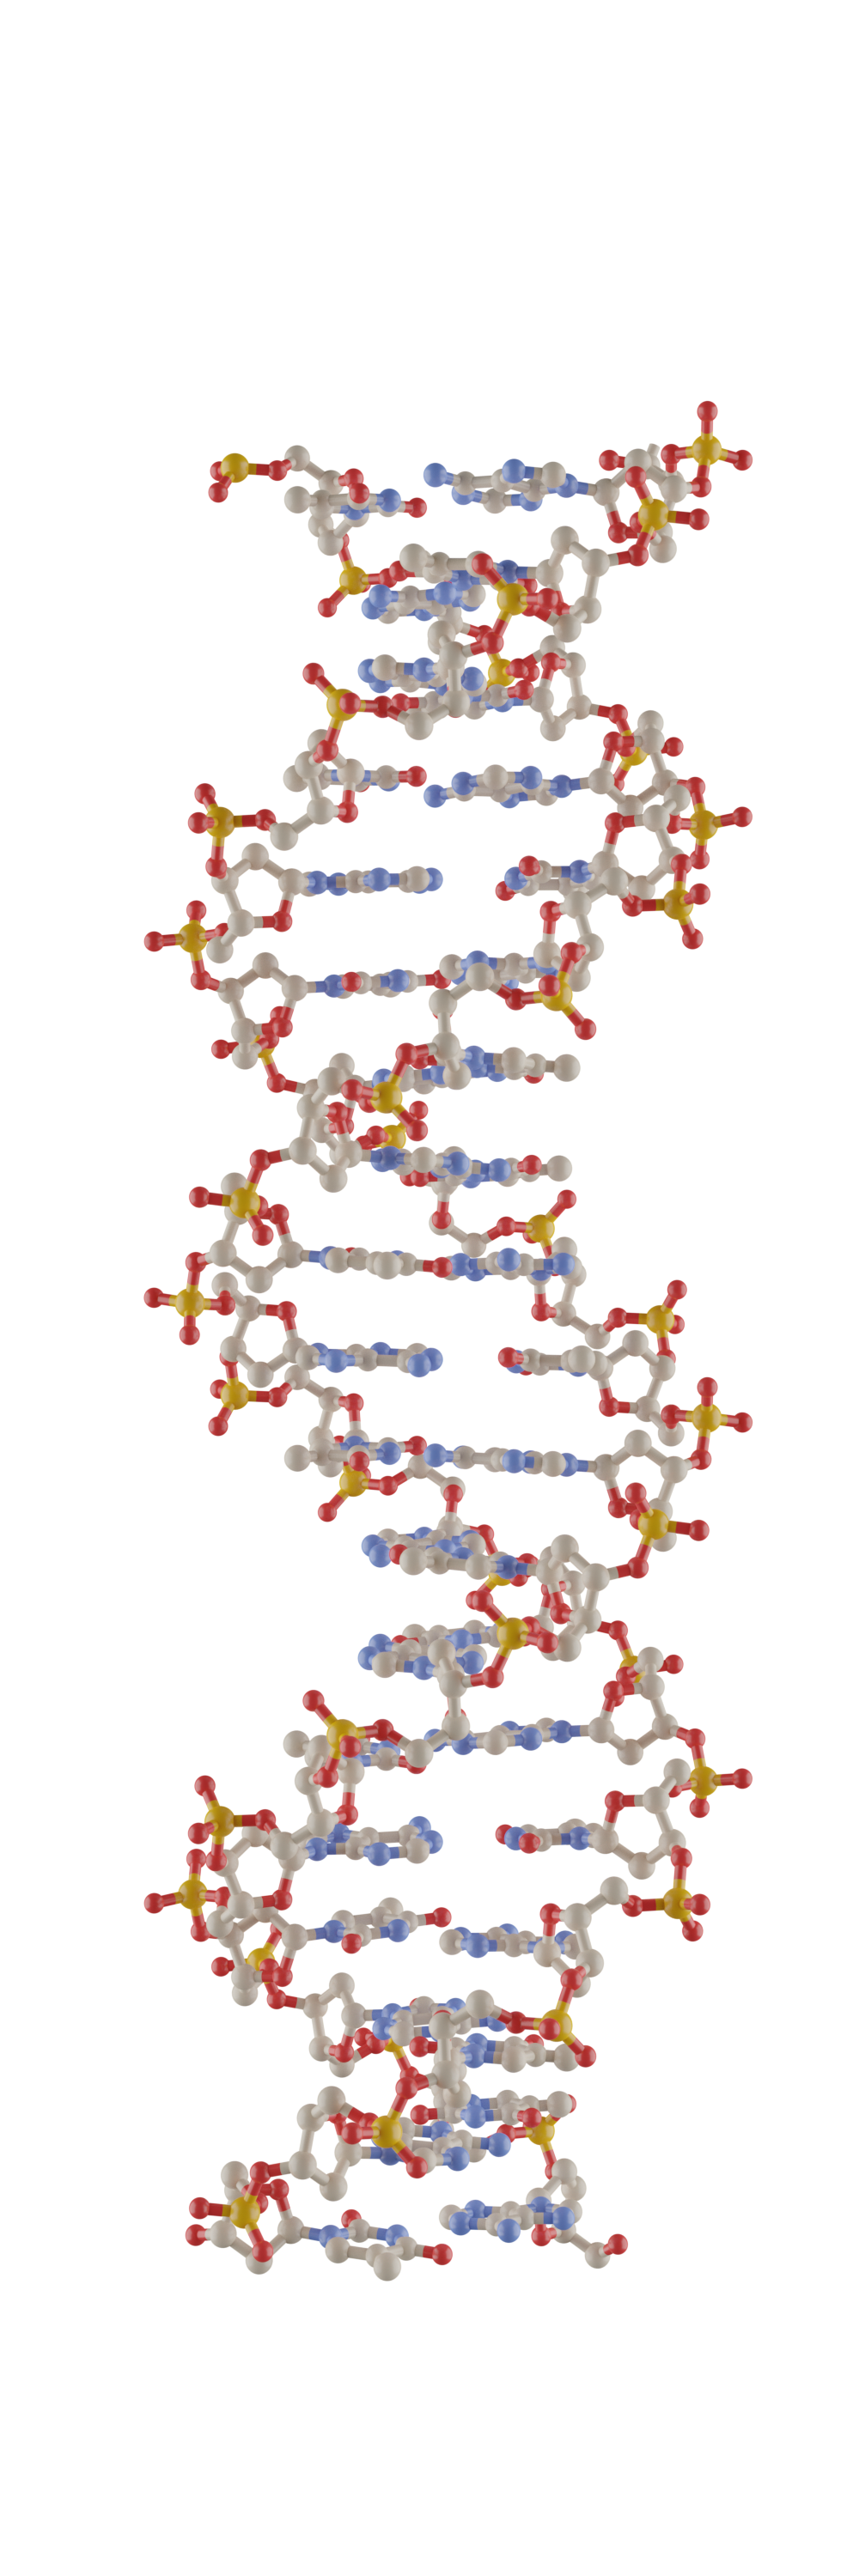
\includegraphics[width=.9\linewidth,valign=t]{Figures/ballnstick.png}
  \end{subfigure}%
  \adjustbox{minipage=1.3em,valign=t}{\subcaption{}\label{sfig:testa}}%
  \begin{subfigure}[t]{\dimexpr.3\linewidth-1.3em\relax}
  \centering
  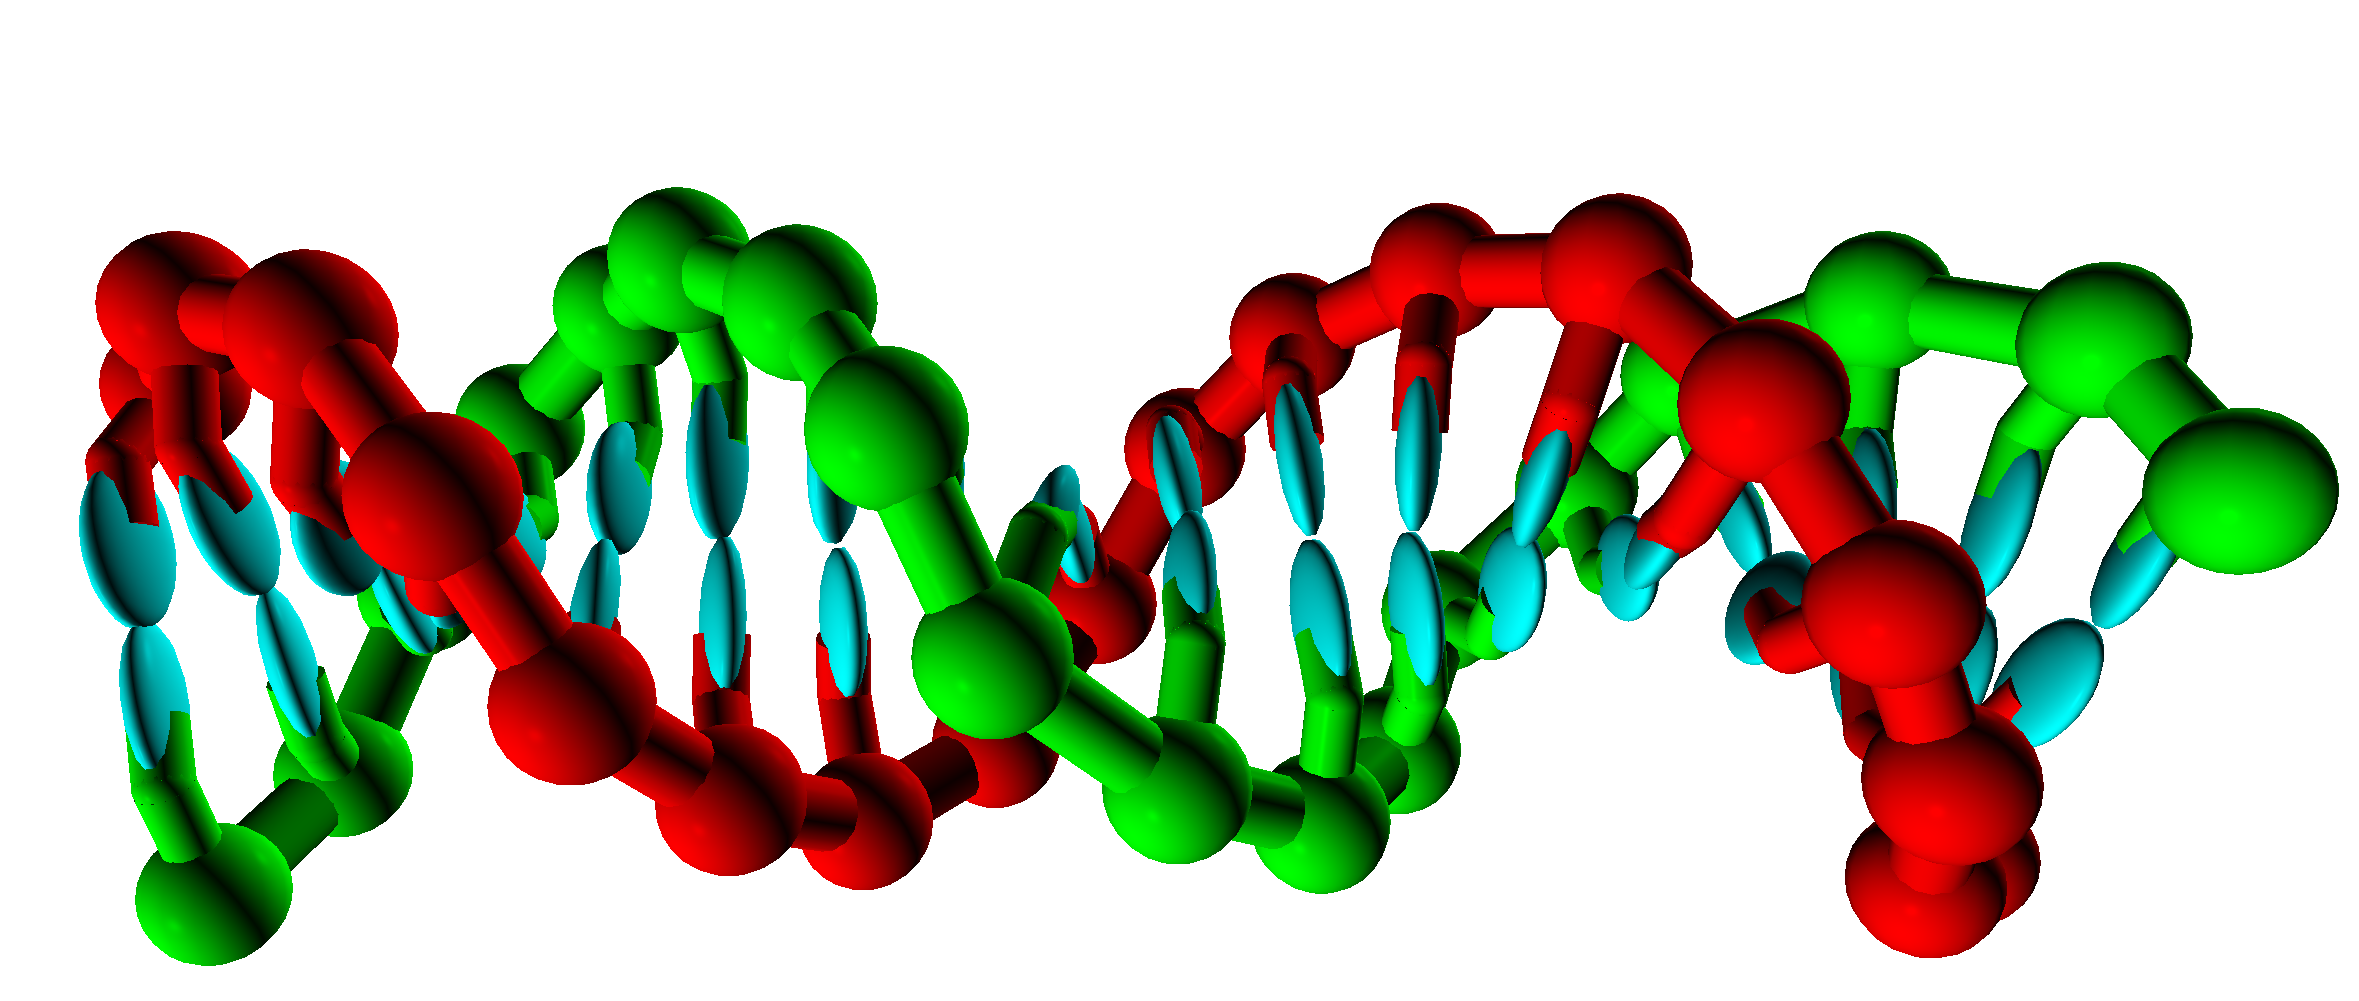
\includegraphics[width=.67\linewidth,valign=t]{Figures/oxDNA.png}
  \end{subfigure}%
  \adjustbox{minipage=1.3em,valign=t}{\subcaption{}\label{sfig:testb}}%
  \begin{subfigure}[t]{\dimexpr.25\linewidth-1.3em\relax}
  \centering
  \vspace{-0.5cm}
  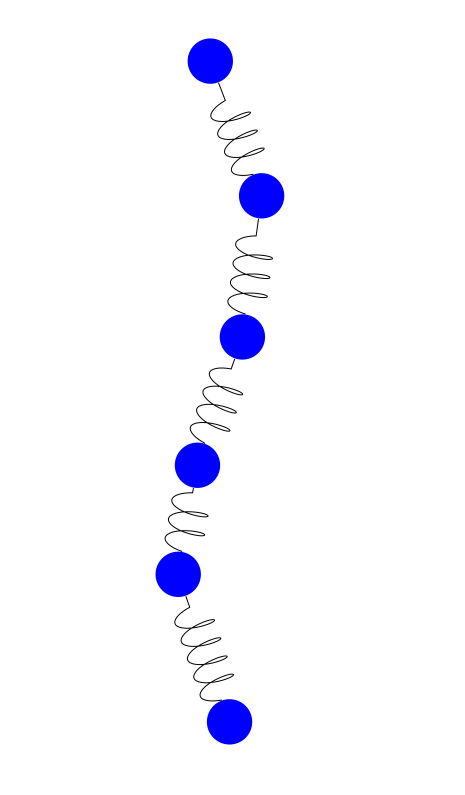
\includegraphics[width=.5\linewidth,valign=t]{Figures/beadSpring.png}
  \end{subfigure}
  \caption[Comparing different degrees of coarse graining DNA]{\linespread{0.816}{\small
    Comparing different coarse-grained models of DNA.  (a) The
    most evident model is of course the All-atom model, providing an atomic description
    of the DNA strand. (b) A second model called OxDNA utilises the individual
    nucleotides as pseudo-atoms, thereby reducing the complexity while preserving much of
    the DNA structure. (c) Further increasing the level of coarse-graining leads to
simplified polymer models, as the bead-and-spring model shown here. The double helix
structure of DNA is not incorporated in this type of model, allowing only for the large
scale behaviour to be studied.}}
    \label{fig:coare-graining}
  \end{centering}
\end{figure}
